
\chapter{New applications using 0.8}
\label{ch:074applications}

\section{Baseline models}
\label{sec:baselineMapping}

Hansson model \cite{Hansson:2013yq} is a complex model
and particularly interesting from the interoperability perspective. 
It contains number of component, both continuous and discrete, such as 
\begin{itemize}
\item 
Biomarker model -- ODEs and algebraic equations 
\item
Model for tumor growth inhibition -- ODEs and algebraic equations 
including a baseline model, based on \cite{dansirikul2008approaches}
\item
Dropout model -- logistic regression model (simulation only)
\item
Survival model -- time-to-event data model 
\end{itemize}
Here we discuss the baseline model because of its structure not
discussed so far in any of the use cases. It requires the implementation of
mapping of the dependent variable at time t=0.
The NMTRAN code for the baseline model elements reads
\lstset{language=NM}
\begin{lstlisting}
	 IF(TIME.EQ.0.AND.FLAG.EQ.4)THEN
	   OBASE  =    DV                        		; observed tumor size at baseline (T= 0)
	 ENDIF
	
	 W1       =    THETA(4)*OBASE
	 IBASE    =    OBASE+ETA(5)*W1		; observed tumor size at baseline acknowledging residual error
	 ...
	 A_0(4) = IBASE                            ; TUMOR
	 
\end{lstlisting}
PharmML implementation of the baseline is done in two steps, first
by declaring the variable (could also be declared as covariate), i.e.
\lstset{language=XML}
\begin{lstlisting}
            <ct:Variable symbolType="real" symbId="OBASE"/>
\end{lstlisting}
which then can be mapped to the dependent variable, DV, column in the
dataset conditional on TIME==0 as the following snippet shows
\lstset{language=XML}
\begin{lstlisting}
    <ColumnMapping>
        <ColumnRef xmlns="http://www.pharmml.org/pharmml/0.7/Dataset" columnIdRef="DV"/>
        <Piecewise xmlns="http://www.pharmml.org/pharmml/0.7/Dataset">
            <math:Piece>
                <ct:SymbRef blkIdRef="sm1" symbIdRef="OBASE"/>
                <math:Condition>
                    <math:LogicBinop op="eq">
                        <ColumnRef columnIdRef="TIME"/>
                        <ct:Real>0</ct:Real>
                    </math:LogicBinop>
                </math:Condition>
            </math:Piece>
        </Piecewise>
    </ColumnMapping>
\end{lstlisting}
Once this is done, the variable OBASE can be used to define the 
initial condition for the tumor growth variable defined by an ODE, $A4$,
\begin{align}
\frac{A4}{dt} &= \mbox{KG} \mbox{A4}-[\mbox{AUC1}+(-\mbox{SKIT})+(-\mbox{VEG3})] \exp(-(\mbox{LAMBDA}\times \mbox{T}))\mbox{A4} \nonumber \\
A4(t=0)	& = \mbox{IBASE} = \mbox{OBASE}+\mbox{ETA(5)}*\mbox{W1} \nonumber % + \mbox{W1}\times \eta_5 \nonumber \\
% \mbox{with} \quad W1 & = \mbox{THETA4} \times \mbox{OBASE} \nonumber
\end{align}


\lstset{language=XML}
\begin{lstlisting}
    <ct:Variable symbolType="real" symbId="W1">
        <ct:Assign>
            <math:Binop op="times">
                <ct:SymbRef blkIdRef="pm1" symbIdRef="theta4"/>
                <ct:SymbRef symbIdRef="OBASE"/>
            </math:Binop>
        </ct:Assign>
    </ct:Variable>
    
    <!-- initial condition value, IBASE -->
    <!-- IBASE = A4(t=0) = OBASE+ETA(5)*W1 -->
    <ct:Variable symbolType="real" symbId="IBASE">
        <ct:Assign>
            <math:Binop op="plus">
                <ct:SymbRef blkIdRef="sm1" symbIdRef="OBASE"/>
                <math:Binop op="times">
                    <ct:SymbRef symbIdRef="W1"/>
                    <ct:SymbRef blkIdRef="pm1" symbIdRef="eta5"/>
                </math:Binop>
            </math:Binop>
        </ct:Assign>
    </ct:Variable>
    
    <!-- dA4/dt -->
    <ct:DerivativeVariable symbolType="real" symbId="A4">
        <ct:Assign>
            <!-- skipped RHS expression: -->
            <!-- KG*A(4)-[AUC1+(-SKIT)+(-VEG3)]*EXP(-(LAMBDA*T))*A(4) -->
        </ct:Assign>
        <ct:InitialCondition>
            <ct:InitialValue>
                <ct:Assign>
                    <ct:SymbRef blkIdRef="pm1" symbIdRef="IBASE"/>
                </ct:Assign>
            </ct:InitialValue>
            <ct:InitialTime>
                <ct:Assign><ct:Real>0</ct:Real></ct:Assign>
            </ct:InitialTime>
        </ct:InitialCondition>
    </ct:DerivativeVariable>
\end{lstlisting}


%\section{Mapping overview}
%\label{sec:mappingOverview}
%example4\_NONMEM.xml
%\lstset{language=XML}
%\begin{lstlisting}
%            <ColumnMapping>
%                <ds:ColumnRef columnIdRef="OCC"/>
%                <ct:SymbRef blkIdRef="cm1" symbIdRef="Occasion"/>
%                <ds:CategoryMapping>
%                    <ds:Map modelSymbol="occ1" dataSymbol="1"/>
%                    <ds:Map modelSymbol="occ2" dataSymbol="2"/>
%                </ds:CategoryMapping>
%            </ColumnMapping>
%\end{lstlisting}
%
%\begin{figure}[ht!]
%\centering
%  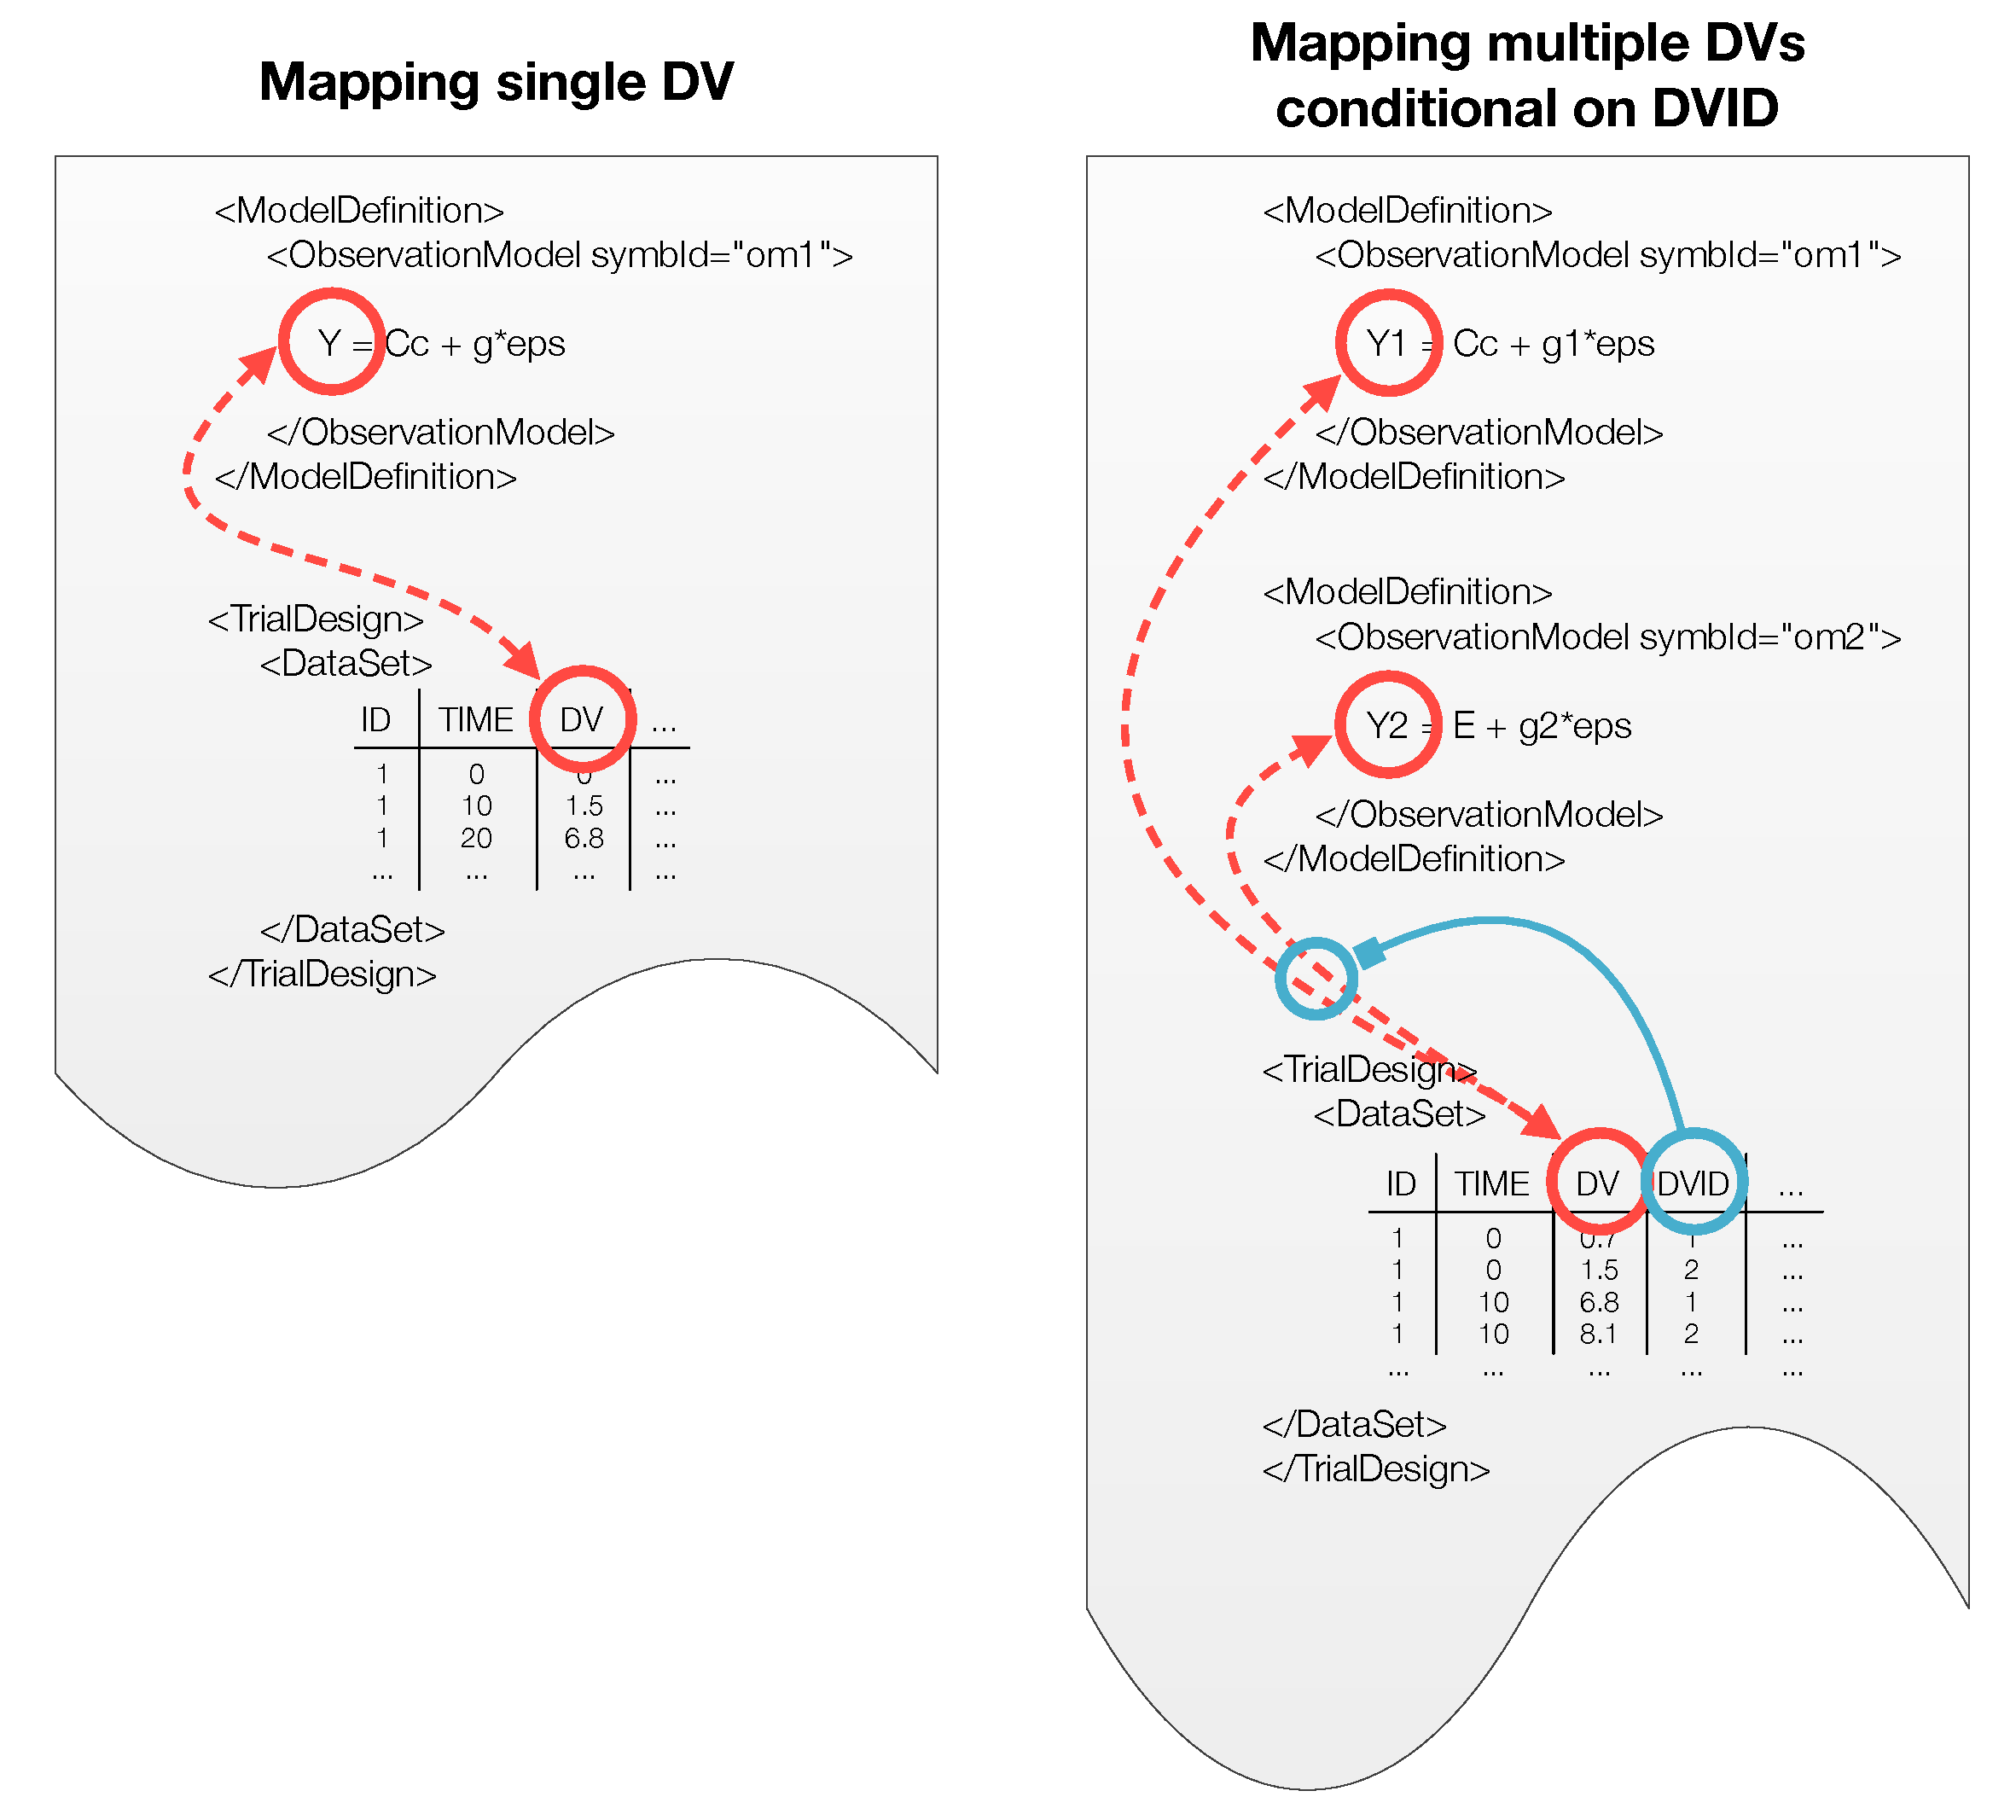
\includegraphics[width=120mm]{pics/mapping1.pdf}
% \caption{....}
% \label{fig:mappingDV}
%\end{figure}


\section{Markov models}
\label{sec:markovModels}
Stimulated by the recent discussion on the DDMoRe forum around Markov 
models\footnote{http://www.ddmore.eu/forum/pharmml-and-sbml}
two examples are discussed with a detailed description and implementation.

It turns out that Markov models, beyond for example disease modelling demonstrated 
in the 2$^{nd}$ example, have other quite unexpected yet relevant application such as zombie 
attack modelling. These attacks have been documented in well-known movies 
such as \emph{Shaun of the Dead} although there many who see this as pure science
fiction. Nevertheless it is a very educational use case described in the first example.

\subsection{Example 1 -- Zombie attack}
\label{subsec:exp1}
The following basic zombie attack model is based on an example in lecture 
notes on Markov Models\footnote{http://www.poritz.net/jonathan/matvec/markov.html}.
Its extension to that shown on the front page of this specification is straightforward.
Other more advanced models are available as well, e.g. \cite{munz2009zombies}, 
\cite{witkowski2013bayesian}, \cite{woolley2014long}.

\begin{figure}[ht!]
\centering
  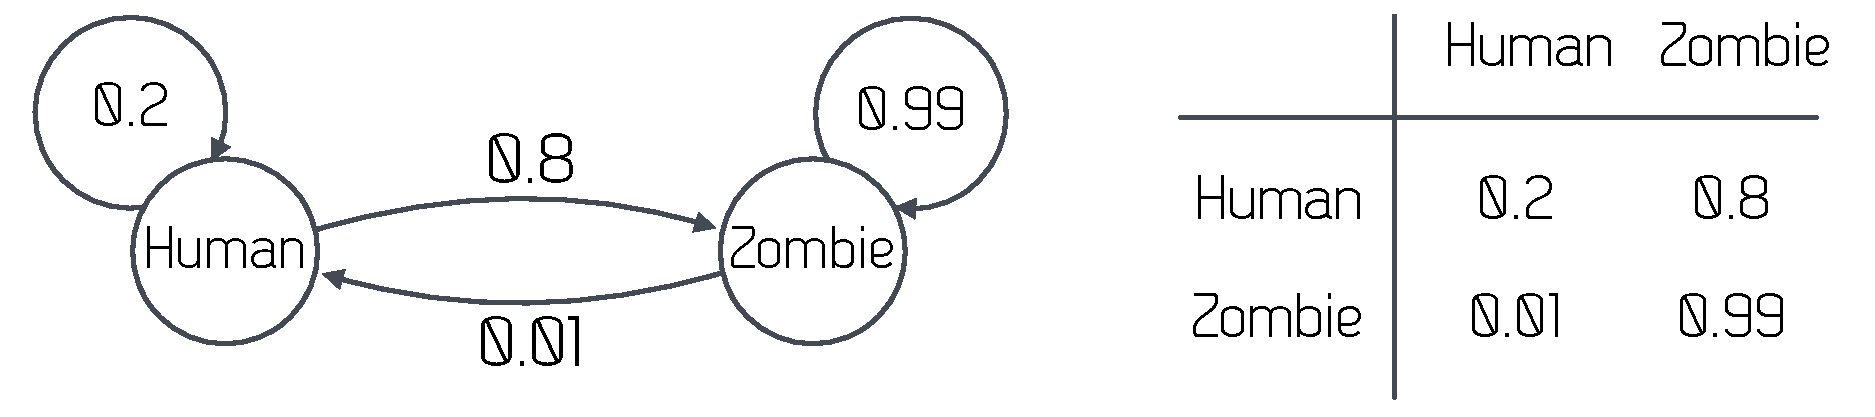
\includegraphics[width=120mm]{pics/MarkovZombie.pdf}
 \caption{Basic Markov model for zombie attack.}
 \label{fig:MarkovZombie}
\end{figure}


\subsection*{Model definition}
\subsubsection*{Observation model}

\begin{itemize}
\item
Type of observed variable -- discrete / categorical
\item
Category variable: $Y$
\item
Initial state variable: $Y_{init}$
\item
Set of categories: $\{\mbox{Human}, \mbox{Zombie}\}$
\item
Transition probabilities
\begin{itemize}
\item
as pairwise conditional transition probabilities
\begin{align}
& P(\mbox{Human} \rightarrow \mbox{Zombie}) = 0.8 \nonumber \\
& P(\mbox{Zombie} \rightarrow \mbox{Human}) = 0.01 \nonumber \\
& P(\mbox{Human} \rightarrow \mbox{Human}) = 0.2 \nonumber \\
& P(\mbox{Zombie} \rightarrow \mbox{Zombie}) = 0.99 \nonumber
\end{align}
\item
or as transition (aka stochastic) matrix
\[
\begin{blockarray}{ccc}
& H & Z \\
\begin{block}{c[cc]}
H &    0.1 & 0.8  \\
Z &    0.01 & 0.99  \\
\end{block}
\end{blockarray}
\]
\end{itemize}
\end{itemize}

\subsection*{Trial Design}

\begin{itemize}
\item
Observations: Y at t=1,...,12 (months).
\end{itemize}


\subsection*{Modelling steps}

\begin{itemize}
\item
Initial states
\begin{align}
& Y_{init} = \left( \begin{array}{c} 100 \\ 0 \end{array} \right) \nonumber
\end{align}
\end{itemize}


\subsubsection*{PharmML implementation}

\lstset{language=XML}
\begin{lstlisting}
    <ModelDefinition xmlns="http://www.pharmml.org/pharmml/0.8/ModelDefinition">
        <!-- OBSERVATIONS -->
        <ObservationModel blkId="om1">
            <Discrete>
                <CategoricalData>
                    
                    <ListOfCategories> 
                        <Category symbId="Human"/>
                        <Category symbId="Zombie"/>
                    </ListOfCategories>
                    
                    <CategoryVariable symbId="Y"/>
                    <InitialStateVariable symbId="Yinit"/> 
                    <PreviousStateVariable symbId="Yp"/>
                    <Dependance type="discreteMarkov"/>
                    
                    <TransitionMatrix type="leftStochastic">
                        <ct:Matrix matrixType="Any">
                            <ct:RowNames>
                                <ct:SymbRef symbIdRef="Human"/><ct:SymbRef symbIdRef="Zombie"/>
                            </ct:RowNames>
                            <ct:MatrixRow>
                                <ct:Real>0.2</ct:Real><ct:Real>0.8</ct:Real>
                            </ct:MatrixRow>
                            <ct:MatrixRow>
                                <ct:Real>0.01</ct:Real><ct:Real>0.99</ct:Real>
                            </ct:MatrixRow>
                        </ct:Matrix>
                    </TransitionMatrix>
                    
                    <!-- ALTERNATIVELY usign Pairwise probabilities -->
                    <!-- P(Y=Zombie|Yp=Human)=0.8 -->
                    <ProbabilityAssignment>
                        <Probability symbId="p1">
                            <CurrentState>
                                <math:LogicBinop op="eq">
                                    <ct:SymbRef symbIdRef="Y"/>
                                    <ct:SymbRef symbIdRef="Zombie"/>
                                </math:LogicBinop>
                            </CurrentState>
                            <PreviousState>
                                <math:LogicBinop op="eq">
                                    <ct:SymbRef symbIdRef="Yp"/>
                                    <ct:SymbRef symbIdRef="Human"/>
                                </math:LogicBinop>
                            </PreviousState>
                        </Probability>
                        <ct:Assign>
                            <ct:Real>0.8</ct:Real>
                        </ct:Assign>
                    </ProbabilityAssignment>
                    <!-- other probabilities analog - skipped here -->
                    
                </CategoricalData>
            </Discrete>
        </ObservationModel>
    </ModelDefinition>
\end{lstlisting}
Trial design: output of variable $Y$ at t=1,...,12 (months).
\lstset{language=XML}
\begin{lstlisting}
    <!-- OBSERVATION DEFINITION: Number of humans/zombies for months 1-12 -->
    <TrialDesign xmlns="http://www.pharmml.org/pharmml/0.8/TrialDesign">
        <Observations>
            <Observation oid="obsOid">
                <ObservationTimes>
                    <ct:Assign>
                        <ct:Sequence>
                            <ct:Begin>
                                <ct:Real>1</ct:Real>
                            </ct:Begin>
                            <ct:StepSize>
                                <ct:Real>1</ct:Real>
                            </ct:StepSize>
                            <ct:End>
                                <ct:Real>12</ct:Real>
                            </ct:End>
                        </ct:Sequence>
                    </ct:Assign>
                </ObservationTimes>
                <Discrete>
                    <ct:SymbRef blkIdRef="om1" symbIdRef="Y"/>
                </Discrete>
            </Observation>
        </Observations>
    </TrialDesign>
\end{lstlisting}
Modelling step definition and initial assignments, $Y_{init} = (100, 0)$
\lstset{language=XML}
\begin{lstlisting}
    <mstep:ModellingSteps>
        <mstep:SimulationStep oid="simOid">
            
            <mstep:ObservationsReference>
                <ct:OidRef oidRef="obsOid"/>
            </mstep:ObservationsReference>
            
            <ct:VariableAssignment>
                <ct:SymbRef blkIdRef="om1" symbIdRef="Yinit"/>
                <ct:Assign>
                    <ct:Vector>
                        <ct:VectorElements>
                            <ct:Real>100</ct:Real>
                            <ct:Real>0</ct:Real>
                        </ct:VectorElements>
                    </ct:Vector>
                </ct:Assign>
            </ct:VariableAssignment>
            
            <mstep:Operation order="1" opType="Number of humans/zombies for months 1-12"/>
        </mstep:SimulationStep>
    </mstep:ModellingSteps>
\end{lstlisting}


\subsubsection{Zombies and epidemiology}
Zombies attack modelling is more then just fun application of mathematics and
has close parallels to epidemiological modelling -- the zombies are walking 
representations of a contagion. 
See for more on: \url{http://www.livescience.com/38527-surviving-a-zombie-apocalypse-math.html}


\subsection{Example 2 -- HIV model}
\label{subsec:exp3}
The second example is based on the published model \cite{Lee:2014kq}
and describes Markov chain modelling analysis of HIV/AIDS progression.
Figure \ref{fig:Markov_HIV} shows the four states  
\begin{itemize}
\item 
S1 -- vulnerable
\item 
S2 -- HIV infective
\item 
S3 -- clinical AIDS persons
\item 
S4 -- death
\end{itemize}
model and the according transition matrix which is \emph{Race} dependent.

\begin{figure}[ht!]
\centering
  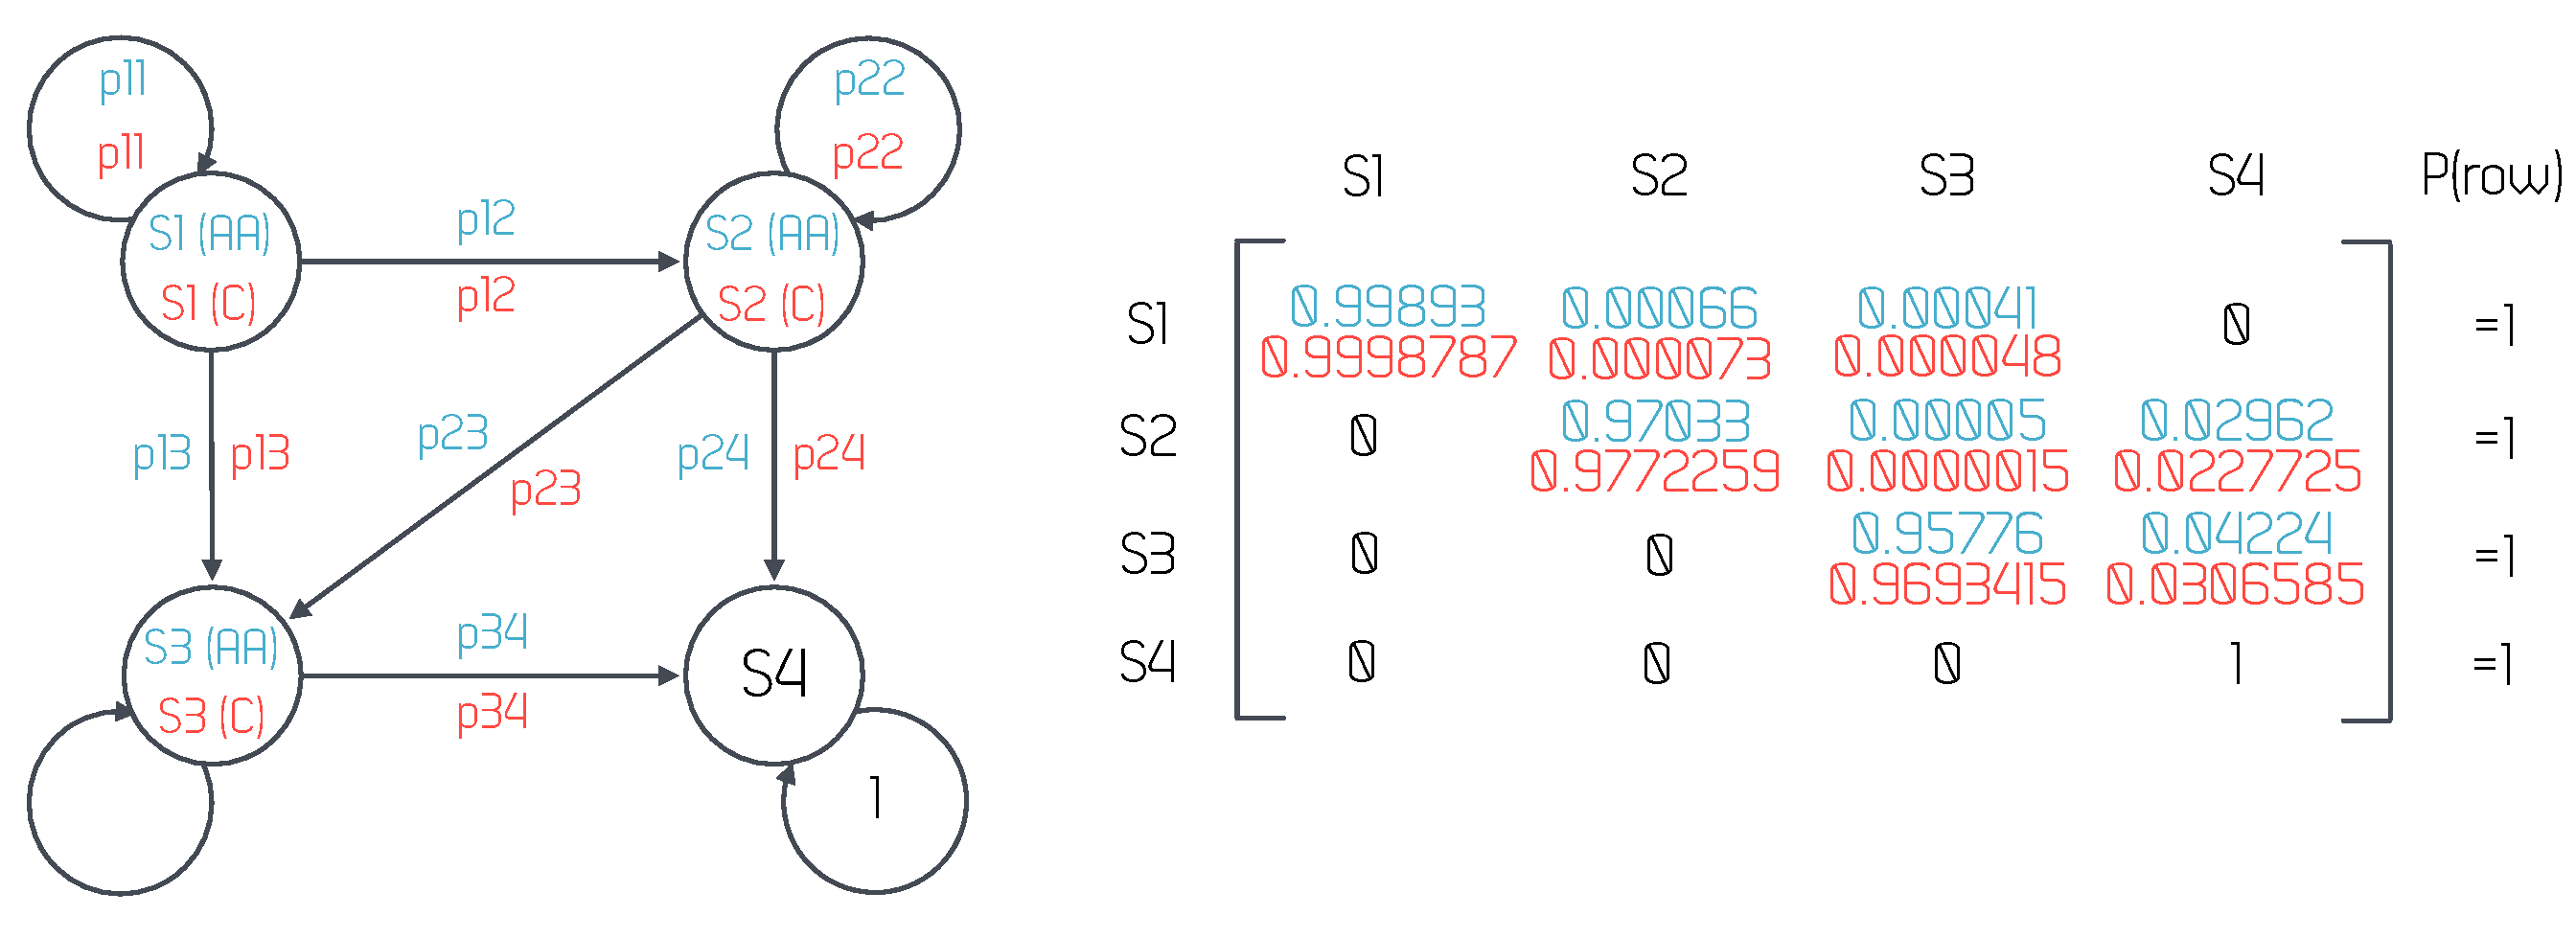
\includegraphics[width=140mm]{pics/Markov_HIV.pdf}
 \caption{Markov model of HIV/AIDS progression.}
 \label{fig:Markov_HIV}
\end{figure}

\subsection*{Model definition}

\subsubsection*{Covariate model}
\begin{itemize}
\item
Race = \{African Americans (AA), Caucasians (C)\} -- categorical covariate
\end{itemize}

\subsubsection*{Observation model}

\begin{itemize}
\item
Type of observed variable -- discrete / categorical
\item
Category variable: $Y$
\item
Initial state variable: $Y_{init}$
\item
Set of categories: $\{\mbox{S1}, \mbox{S2}, \mbox{S3}, \mbox{S4}\}$
\item
Transition probabilities
\begin{itemize}
\item
as pairwise conditional transition probabilities
\begin{align}
& P(\mbox{S1} \rightarrow \mbox{S1} | \; Race==AA) = 0.99893 \nonumber \\
& P(\mbox{S1} \rightarrow \mbox{S1} | \; Race==C) = 0.9998787 \nonumber \\
& P(\mbox{S1} \rightarrow \mbox{S2} | \; Race==AA) = 0.00066 \nonumber \\
& P(\mbox{S1} \rightarrow \mbox{S2} | \; Race==C) = 0.000073 \nonumber \\
& P(\mbox{S1} \rightarrow \mbox{S3} | \; Race==AA) = 0.00041 \nonumber \\
& P(\mbox{S1} \rightarrow \mbox{S3} | \; Race==C) = 0.000048 \nonumber \\
& P(\mbox{S1} \rightarrow \mbox{S4}) = 0 \nonumber \\
& \mbox{other probabilities follow from the property 'left stochastic matrix'} \nonumber
\end{align}
\item
or as transition (aka stochastic) matrix -- see Figure \ref{fig:Markov_HIV} (right)
\end{itemize}
\end{itemize}

\subsection*{Trial Design}

\begin{itemize}
\item
Observations: Y at t=1,...,10 (years).
\item
Covariates: Race={AA, C, AA, C, \dots, AA, C}.
\end{itemize}

\subsection*{Modelling steps}

\begin{itemize}
\item
Initial states
\begin{align}
& Y_{init} = \left( \begin{array}{c} 100 \\ 0 \\ 0 \\ 0 \end{array} \right) \nonumber
\end{align}
\end{itemize}

\subsubsection*{PharmML implementation}

\begin{itemize}
\item
Covariate Model 
\lstset{language=XML}
\begin{lstlisting}
<ModelDefinition xmlns="http://www.pharmml.org/pharmml/0.8/ModelDefinition">
    
    <!-- Covariate Model -->
    <CovariateModel blkId="cm1">
        <Covariate symbId="RACE">
            <Categorical>
                <Category catId="AA"/>
                <Category catId="C"/>
            </Categorical>
        </Covariate>
    </CovariateModel>
\end{lstlisting}

\item
Observation Model with transition matrix -- we use the fact that a matrix element 
can contain an arbitrary expression, also a piecewise function used here for the 
transition probability from the \emph{S1} to \emph{S1}, \emph{S2}, \dots, 
\emph{S4} states conditioned on the covariate \emph{Race}. 
\lstset{language=XML}
\begin{lstlisting}    
    <!-- Observation Model -->
    <ObservationModel blkId="om1">
        <Discrete>
            <CategoricalData>
                
                <ListOfCategories> 
                    <Category symbId="S1"/>
                    <Category symbId="S2"/>
                    <Category symbId="S3"/>
                    <Category symbId="S4"/>
                </ListOfCategories>
                
                <CategoryVariable symbId="Y"/>
                
                <InitialStateVariable symbId="Yinit"/> 
                <PreviousStateVariable symbId="Yp"/>
                
                <Dependance type="discreteMarkov"/>
                
                <TransitionMatrix type="leftStochastic">
                    <ct:Matrix matrixType="Any">
                        <ct:RowNames>
                            <ct:SymbRef symbIdRef="S1"/>
                            <ct:SymbRef symbIdRef="S2"/>
                            <ct:SymbRef symbIdRef="S3"/>
                            <ct:SymbRef symbIdRef="S4"/>
                        </ct:RowNames>
                        <ct:MatrixRow>
                            <ct:Assign>
                                <ct:Piecewise>
                                    <math:Piece>
                                        <ct:Real>0.99893</ct:Real>
                                        <math:Condition>
                                            <math:LogicBinop op="eq">
                                                <ct:SymbRef symbIdRef="RACE"/>
                                                <ct:CatRef catIdRef="AA"/>
                                            </math:LogicBinop>
                                        </math:Condition>
                                    </math:Piece>
                                    <math:Piece>
                                        <ct:Real>0.9998787</ct:Real>
                                        <math:Condition>
                                            <math:LogicBinop op="eq">
                                                <ct:SymbRef symbIdRef="RACE"/>
                                                <ct:CatRef catIdRef="C"/>
                                            </math:LogicBinop>
                                        </math:Condition>
                                    </math:Piece>
                                </ct:Piecewise>
                            </ct:Assign>
                            <ct:Assign>
                                <ct:Piecewise>
                                    <math:Piece>
                                        <ct:Real>0.00066</ct:Real>
                                        <math:Condition>
                                            <math:LogicBinop op="eq">
                                                <ct:SymbRef symbIdRef="RACE"/>
                                                <ct:CatRef catIdRef="AA"/>
                                            </math:LogicBinop>
                                        </math:Condition>
                                    </math:Piece>
                                    <math:Piece>
                                        <ct:Real>0.000073</ct:Real>
                                        <math:Condition>
                                            <math:LogicBinop op="eq">
                                                <ct:SymbRef symbIdRef="RACE"/>
                                                <ct:CatRef catIdRef="C"/>
                                            </math:LogicBinop>
                                        </math:Condition>
                                    </math:Piece>
                                </ct:Piecewise>
                            </ct:Assign>
                            <ct:Assign>
                                <ct:Piecewise>
                                    <math:Piece>
                                        <ct:Real>0.00041</ct:Real>
                                        <math:Condition>
                                            <math:LogicBinop op="eq">
                                                <ct:SymbRef symbIdRef="RACE"/>
                                                <ct:CatRef catIdRef="AA"/>
                                            </math:LogicBinop>
                                        </math:Condition>
                                    </math:Piece>
                                    <math:Piece>
                                        <ct:Real>0.000048</ct:Real>
                                        <math:Condition>
                                            <math:LogicBinop op="eq">
                                                <ct:SymbRef symbIdRef="RACE"/>
                                                <ct:CatRef catIdRef="C"/>
                                            </math:LogicBinop>
                                        </math:Condition>
                                    </math:Piece>
                                </ct:Piecewise>
                            </ct:Assign>
                            <ct:Real>0</ct:Real>
                        </ct:MatrixRow>
                        <ct:MatrixRow>
                            <!-- 2nd row skipped -->
                        </ct:MatrixRow>
                        <ct:MatrixRow>
                            <!-- 3rd row skipped -->
                        </ct:MatrixRow>
                        <ct:MatrixRow>
                            <ct:Real>0</ct:Real><ct:Real>0</ct:Real><ct:Real>0</ct:Real><ct:Real>1</ct:Real>
                        </ct:MatrixRow>
                    </ct:Matrix>
                </TransitionMatrix>
\end{lstlisting}
\item
Trial design
\begin{itemize}
\item 
Output of variable $Y$ at t=1,...,10 (years).
\item 
Covariates: Race={AA, C, AA, C, \dots, AA, C}.
\end{itemize}
\lstset{language=XML}
\begin{lstlisting}
    <TrialDesign xmlns="http://www.pharmml.org/pharmml/0.8/TrialDesign">

	<!-- <Observations> skipped as identical to that in previous example -->
        
        <Covariates>
            <IndividualCovariates>
                <ColumnMapping>
                    <ds:ColumnRef columnIdRef="race"/>
                    <ct:SymbRef blkIdRef="cm1" symbIdRef="RACE"/>
                </ColumnMapping>
                <ds:DataSet>
                    <ds:Definition>
                        <ds:Column columnId="ID" valueType="string" columnNum="1"/>
                        <ds:Column columnId="race" valueType="string" columnNum="2"/>
                    </ds:Definition>
                    <ds:Table>
                        <ds:Row><ct:String>1</ct:String><ct:String>AA</ct:String></ds:Row>
                        <ds:Row><ct:String>2</ct:String><ct:String>C</ct:String></ds:Row>
                        <ds:Row><ct:String>3</ct:String><ct:String>AA</ct:String></ds:Row>
                        <ds:Row><ct:String>4</ct:String><ct:String>C</ct:String></ds:Row>
                        <ds:Row><ct:String>5</ct:String><ct:String>AA</ct:String></ds:Row>
                        <!-- subject omitted -->
                        <ds:Row><ct:String>99</ct:String><ct:String>AA</ct:String></ds:Row>
                        <ds:Row><ct:String>100</ct:String><ct:String>C</ct:String></ds:Row>
                    </ds:Table>
                </ds:DataSet>
            </IndividualCovariates>
        </Covariates>
    </TrialDesign>
\end{lstlisting}
\item
Modelling step definition is omitted as analog to those in the previous example.
\end{itemize}


\subsection{Out of scope}
Compared to the discussion on the DDMoRe forum website around the Markov models
not all requested features, especially around the task execution, are covered by this
PharmML version. 
From the start we have focused on a declarative model description and
don't cover many structures featured in a typical programming language.

Nevertheless, additional features could be build in into the format both on 
model definition and task description side. It will require an additional discussion 
and well defined requirements to cover them if needed.


%\section{Multiple infusions}
%
%Alternatively, you could use DesignParameter to encode the 
%amount vector
%\lstset{language=XML}
%\begin{lstlisting}
%		<mdef:DesignParameter symbId="doseAmountVector">
%			<ct:Assign>
%				<ct:Vector>
%					<ct:VectorElements>
%						<ct:Real>1</ct:Real>
%						<ct:Real>2</ct:Real>
%						<ct:Real>1</ct:Real>
%						<ct:Real>5</ct:Real>
%						<!-- ... -->
%					</ct:VectorElements>
%				</ct:Vector>
%			</ct:Assign>
%		</mdef:DesignParameter>
%\end{lstlisting}
%
%and then refer to it in (see in bold below)
%\lstset{language=XML}
%\begin{lstlisting}
%	<Interventions>
%		<Administration oid="inf1">
%			<Infusion>
%				<DoseAmount>
%					<ct:SymbRef symbIdRef="Ad"/>
%					<ct:Assign>
%						<math:Binop op="divide">
%							<math:Binop op="times">
%								<ct:SymbRef symbIdRef="doseAmountVector"/>
%								<ct:SymbRef blkIdRef="mmcvt" symbIdRef="wgt" />
%							</math:Binop>
%							<ct:SymbRef blkIdRef="mmpar" symbIdRef="V" />
%						</math:Binop>
%					</ct:Assign>
%				</DoseAmount>
%				<DosingTimes>
%					<ct:Assign>
%						<ct:Vector>
%							<ct:VectorElements>
%								<ct:Real>0</ct:Real>
%								<ct:Real>5</ct:Real>
%								<ct:Real>10</ct:Real>
%								<!-- ... -->
%							</ct:VectorElements>
%						</ct:Vector>
%					</ct:Assign>
%				</DosingTimes>
%				<Rate>
%					<ct:Assign>
%						<ct:Vector>
%							<ct:VectorElements>
%								<ct:Real>10</ct:Real>
%								<ct:Real>15</ct:Real>
%								<ct:Real>20</ct:Real>
%								<!-- ... -->
%							</ct:VectorElements>
%						</ct:Vector>	
%					</ct:Assign>
%				</Rate>
%				ALTERNATIVE 
%				<Duration>
%					<ct:Assign>
%						<ct:Vector>
%							<ct:VectorElements>
%								<ct:Real>10</ct:Real>
%								<ct:Real>15</ct:Real>
%								<ct:Real>20</ct:Real>
%								<!-- ... -->
%							</ct:VectorElements>
%						</ct:Vector>
%					</ct:Assign>
%				</Duration>
%			</Infusion>
%		</Administration>
%\end{lstlisting}
%















